% AY2022 制御工学 解答例
% 回答の流れ・言葉遣いは 03_制御工学/参考/「制御工学Ⅱ（完成版）」に寄せる。
% デザイン（囲み枠等）は真似しない。解答・数値は本年度過去問から自力で導いた。
\documentclass[11pt,a4paper]{article}
\usepackage{../../../00_common/preamble}

\usetikzlibrary{positioning,arrows.meta,calc}
\usepackage{pgfplots}
\pgfplotsset{compat=newest}

\title{制御工学 AY2022 解答例（専門応用科目I）}
\author{}
\date{}

\begin{document}
\maketitle

% ==================================================================
\section*{第1問〔I〕}

壁 $-$ バネ $k$ $-$ 質量 $m$ $-$ ダンパ $d$ $-$ 自由端（入力 $x_1$）の系。$x_2$ は質量の変位。

\subsection*{(1) 運動方程式と伝達関数}
バネは壁と質量を、ダンパは質量と入力端を結ぶ。
\begin{align*}
  &\qquad m\ddot{x}_2=-k x_2+d(\dot{x}_1-\dot{x}_2)
   \quad\therefore\quad (ms^2+ds+k)X_2=ds\,X_1.
\end{align*}
\[
  \therefore\quad \ans{\;G(s)=\dfrac{X_2(s)}{X_1(s)}=\dfrac{ds}{ms^2+ds+k}\;}
\]

\subsection*{(2) ステップ応答（$m=1,d=3,k=2$）}
$G(s)=\dfrac{3s}{(s+1)(s+2)}$、$X_1=\dfrac1s$ より
\begin{align*}
  &\qquad X_2(s)=\frac{3}{(s+1)(s+2)}=\frac{3}{s+1}-\frac{3}{s+2}
   \quad\therefore\quad x_2(t)=3\bigl(\e^{-t}-\e^{-2t}\bigr).
\end{align*}
$s=0$ に零点をもつため定常値は $0$。
\[
  \therefore\quad \ans{\;x_2(t)=3(\e^{-t}-\e^{-2t})\;}
\]

\subsection*{(3) 最大値と発生時間}
\begin{align*}
  &\qquad \dot{x}_2=3(-\e^{-t}+2\e^{-2t})=0
   \quad\therefore\quad 2\e^{-2t}=\e^{-t}
   \quad\therefore\quad \e^{t}=2,\ t=\ln 2.
\end{align*}
このとき $x_2=3\bigl(\tfrac12-\tfrac14\bigr)=\tfrac34$。
\[
  \therefore\quad \ans{\;x_{2\max}=\dfrac34\ \ (t=\ln2\approx0.69)\;}
\]

\subsection*{(4) 減衰正弦入力応答（$m=1,d=2,k=2$、$x_1(t)=\e^{-t}\sin t$）}
$G(s)=\dfrac{2s}{s^2+2s+2}=\dfrac{2s}{(s+1)^2+1}$、$X_1(s)=\mathcal{L}[\e^{-t}\sin t]=\dfrac{1}{(s+1)^2+1}$ より
\begin{align*}
  &\qquad X_2(s)=\frac{2s}{\bigl((s+1)^2+1\bigr)^2}.
\end{align*}
入力の極が系の極 $s=-1\pm j$ と一致する（共振）ため、逆変換は $t$ を含む項をもつ。
\[
  \therefore\quad \ans{\;x_2(t)=\e^{-t}\bigl(t(\sin t+\cos t)-\sin t\bigr)\;}
\]
$\e^{-t}$ が支配するので、充分な時間が経過すると
\[
  \therefore\quad \ans{\;\lim_{t\to\infty}x_2(t)=0\;}
\]

\bigskip
\noindent 検算: (2) は $s=0$ 零点で定常 $0$、(3) は $t=\ln2$ で $x_{2\max}=\tfrac34$、
(4) は $x_2=\e^{-t}(t(\sin t+\cos t)-\sin t)$ で充分時間後 $0$ を SymPy で確認✓。

\newpage
% ==================================================================
\section*{第2問〔II〕}

前向き $G_1G_2$、帰還 $K$ のフィードバック系。$G_1=\dfrac{1}{s+1}$、$G_2=\dfrac{1}{10s+1}$、$K=2$。

\subsection*{(1) 一巡伝達関数のゲインと位相}
一巡伝達関数はループ一周の積 $L(s)=K G_1 G_2=\dfrac{2}{(s+1)(10s+1)}$。$s=j\omega$ として
\[
  \therefore\quad \ans{\;|L(j\omega)|=\dfrac{2}{\sqrt{1+\omega^2}\,\sqrt{1+(10\omega)^2}},\quad
  \angle L(j\omega)=-\tan^{-1}\omega-\tan^{-1}10\omega\;}
\]

\subsection*{(2) ゲイン線図（漸近線）}
$|L(0)|=2$、すなわち $20\log_{10}2\approx6\,\mathrm{dB}$。折れ点は $10s+1$ より $\omega=0.1$、
$s+1$ より $\omega=1\,[\mathrm{rad/s}]$。傾きは $\omega<0.1$ で $0$、$0.1<\omega<1$ で $-20$、
$\omega>1$ で $-40\,[\mathrm{dB/dec}]$。（(4) の場合を破線で併記。）

\begin{center}
\begin{tikzpicture}
\begin{axis}[
  width=0.86\linewidth, height=5.0cm,
  xmin=1e-2, xmax=1e3, ymin=-70, ymax=20, xmode=log,
  xlabel={$\omega\,[\mathrm{rad/s}]$}, ylabel={ゲイン [dB]},
  ytick={-60,-40,-20,0,6,20},
  xmajorgrids=true, ymajorgrids=true, xminorgrids=true,
  grid style={line width=0.3pt, draw=gray!60},
  extra y ticks={0}, extra y tick style={grid=major, grid style={line width=1pt, draw=black}},
  legend pos=south west, clip=true, enlargelimits=false,
]
% (2): DC 6dB, 折れ点 0.1,1
\addplot[thick] coordinates {(0.01,6) (0.1,6) (1,-14) (1000,-134)};
\addlegendentry{(2) $K{=}2,\,G_2{=}\frac{1}{10s+1}$}
% (4): DC 0dB, 折れ点 1,5
\addplot[thick,dashed] coordinates {(0.01,0) (1,0) (5,-14) (1000,-60)};
\addlegendentry{(4) $K{=}1,\,G_2{=}\frac{1}{0.2s+1}$}
\node[anchor=south] at (axis cs:0.1,6) {\scriptsize $0.1$};
\node[anchor=south] at (axis cs:1,6) {\scriptsize $1$};
\node[anchor=north] at (axis cs:5,-14) {\scriptsize $5$};
\end{axis}
\end{tikzpicture}
\end{center}

\subsection*{(3) 単位ステップ応答}
閉ループは
\begin{align*}
  &\qquad T(s)=\frac{G_1G_2}{1+KG_1G_2}
   =\frac{1}{(s+1)(10s+1)+2}=\frac{1}{10s^2+11s+3}=\frac{1}{(2s+1)(5s+3)}.
\end{align*}
極は $s=-0.5,\ -0.6$（過減衰）、定常値 $T(0)=\dfrac13$。$X(s)=\dfrac{T(s)}{s}$ を分解して
\[
  \therefore\quad \ans{\;x(t)=\dfrac13-2\e^{-0.5t}+\dfrac53\e^{-0.6t}\;}
\]

\begin{center}
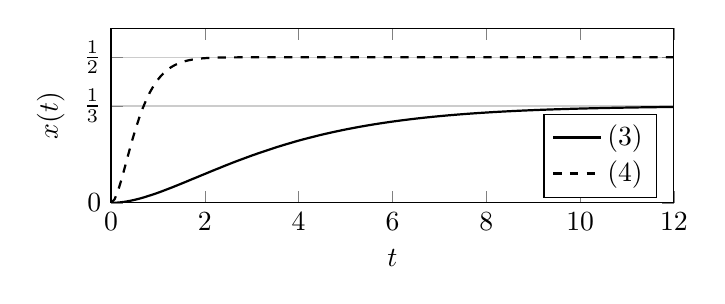
\begin{tikzpicture}
\begin{axis}[
  width=0.72\linewidth, height=3.8cm,
  xmin=0, xmax=12, ymin=0, ymax=0.6,
  xlabel={$t$}, ylabel={$x(t)$},
  ytick={0,0.333,0.5}, yticklabels={$0$,$\frac13$,$\frac12$},
  ymajorgrids=true, grid style={gray!40}, legend pos=south east,
]
\addplot[thick,domain=0:12,samples=120]{1/3-2*exp(-0.5*x)+(5/3)*exp(-0.6*x)};
\addlegendentry{(3)}
\addplot[thick,dashed,domain=0:12,samples=160]{0.5-0.5*exp(-3*x)*(cos(deg(x))+3*sin(deg(x)))};
\addlegendentry{(4)}
\end{axis}
\end{tikzpicture}
\end{center}

\subsection*{(4) $G_2=\dfrac{1}{0.2s+1}$、$K=1$ の場合の比較}
一巡伝達関数は $L(s)=\dfrac{1}{(s+1)(0.2s+1)}$、$|L(0)|=1=0\,\mathrm{dB}$、折れ点 $\omega=1,\ 5$。閉ループは
\begin{align*}
  &\qquad T(s)=\frac{G_1G_2}{1+KG_1G_2}
   =\frac{1}{(s+1)(0.2s+1)+1}=\frac{5}{s^2+6s+10}=\frac{5}{(s+3)^2+1}.
\end{align*}
極は $s=-3\pm j$（不足減衰）、定常値 $T(0)=\dfrac12$。ステップ応答は
\[
  \therefore\quad \ans{\;x(t)=\dfrac12-\dfrac12\e^{-3t}\bigl(\cos t+3\sin t\bigr)\;}
\]
\textbf{考察}：
\begin{itemize}\setlength{\itemsep}{1pt}
  \item \textbf{時間応答}：(3) は実根 $-0.5,-0.6$ の過減衰で整定が遅く無振動。(4) は複素根
        $-3\pm j$ の不足減衰となり、約 10 倍速く立ち上がるが、わずかにオーバーシュートを伴う。
  \item \textbf{ゲイン線図}：$G_2$ の折れ点が $\omega=0.1\to5$ に移って $-20\,$dB/dec の帯が
        高周波側へ広がり、帯域が拡大する。
  \item 定常値は $K$ の違い（$2\to1$）により $\tfrac13\to\tfrac12$ に変わる。
\end{itemize}

\bigskip
\noindent 検算: (1) $L=2/((s+1)(10s+1))$、(3) $T=1/(10s^2+11s+3)$ 極 $\{-0.5,-0.6\}$ 定常 $\tfrac13$、
(4) $T=5/((s+3)^2+1)$ 極 $-3\pm j$ 定常 $\tfrac12$ を SymPy で確認✓。

\end{document}
